\documentclass[a4paper,12pt]{article}
% Package to make citations superscrit with brackets
\usepackage[super,square]{natbib}
% Package to change margin size
\usepackage{anysize}
\marginsize{2cm}{2cm}{1cm}{2cm}
% Package to make headers
\usepackage{fancyhdr}
\renewcommand{\headrulewidth}{0pt}
% Package for highligths
\usepackage{soul}
% Colors for the references links
\usepackage[dvipsnames]{xcolor}
% Package to link references
\usepackage{hyperref}
\usepackage{subcaption}
\hypersetup{
    colorlinks=true,
    linkcolor=black,
    citecolor=CadetBlue,
    filecolor=CadetBlue,      
    urlcolor=CadetBlue,
}
% Package for lorem ipsum
\usepackage{lipsum}
% Package for multicolumn
\usepackage{multicol}
% Package for removing paragraph identations
\usepackage{parskip}
\setlength\columnsep{18pt}
\usepackage{graphicx}
\usepackage[font=small,labelfont=bf]{caption}
\usepackage{amsmath}
\usepackage{siunitx}
\usepackage{titlesec}
\usepackage{listings}
\usepackage{enumitem}
\usepackage{xcolor}
\setcounter{secnumdepth}{4}
\titleformat{\section}[block]{\Large\bfseries\filcenter}{}{1em}{}

\definecolor{codegreen}{rgb}{0,0.6,0}
\definecolor{codegray}{rgb}{0.5,0.5,0.5}
\definecolor{codepurple}{rgb}{0.58,0,0.82}
\definecolor{backcolour}{RGB}{242,242,242}

\lstdefinestyle{mystyle}{
    backgroundcolor=\color{backcolour},   
    commentstyle=\color{codegreen},
    keywordstyle=\color{magenta},
    numberstyle=\tiny\color{codegray},
    stringstyle=\color{codepurple},
    basicstyle=\ttfamily\footnotesize,
    breakatwhitespace=false,         
    breaklines=true,                 
    captionpos=b,                    
    keepspaces=true,                 
    numbers=left,                    
    numbersep=5pt,                  
    showspaces=false,                
    showstringspaces=false,
    showtabs=false,                  
    tabsize=2
}
\lstset{style=mystyle}

% Sets bastract
\renewenvironment{abstract}
 {\par\noindent\textbf{\abstractname}\ \ignorespaces \\}
 {\par\noindent\medskip}



 
\begin{document}
% Makes header
\pagestyle{fancy}
\thispagestyle{empty}
\fancyfoot[R]{\textit{\small https://github.com/lennymalard/melpy-project}}
\fancyfoot[L]{\thepage}`
\fancyfoot[C]{}'
\fancyhead{}
% Makes footnotes with an asterisk
\renewcommand*{\thefootnote}{\fnsymbol{footnote}}
\begin{center}
\Large{\textbf{Implémentation de CNNs avec NumPy}}
\vspace{0.4cm}
\normalsize
\\ Lenny Malard \\
\vspace{0.1cm}
\textit{Melpy Project}
\medskip
\normalsize
\end{center}
{\color{gray}\hrule}
\vspace{0.4cm}
\begin{abstract}
L’implémentation de réseaux de neurones artificiels à partir de zéro constitue un véritable défi 
pédagogique dans l’apprentissage du Deep Learning. Ce processus exige une compréhension approfondie 
des concepts fondamentaux, nécessaire pour transcrire ces connaissances dans la conception d’algorithmes 
optimisés. C’est dans cette optique d'apprentissage que j’ai créé Melpy, une bibliothèque 
de Deep Learning qui, à l’origine, n’implémentait que de simples perceptrons multicouches. C'est donc pourquoi, 
j’ai entrepris d’implémenter les réseaux de neurones convolutifs afin d’étendre les possibilités offertes par 
Melpy et d’enrichir mes connaissances. \\


Étant donné que Melpy repose sur l’utilisation de NumPy, de nouvelles couches spécifiques à ces architectures 
ont été ajoutées et optimisées en exploitant les fonctionnalités de cette bibliothèque. Les résultats obtenus 
montrent que Melpy est désormais capable de produire des performances globalement comparables à celles de Keras, 
dans la classification de jeux de données telles que MNIST et CIFAR-10. Cependant, ces résultats mettent également 
en évidence les limites de de la bibliothèque en termes d’optimisation computationnelle, notamment dû à l'interprétation
du code en Python, ce qui constitue un axe d'amélioration pour l'avenir.
\end{abstract}
\renewcommand{\contentsname}{Table des matières}
{\color{gray}\hrule}
\medskip
\begin{multicols}{2}
\tableofcontents
\section{Introduction}
Les réseaux de neurones convolutifs (CNNs) ont été cités pour 
la première fois par Yann LeCun en 1998, dans le papier 
\textit{“Gradient-Based Learning Applied to Document Recognition”} \cite{YannLeCunCNNs}.
Il y met en avant l’apprentissage automatique des motifs présents dans les 
images d’un jeu de données et démontre l’efficacité du modèle dans des tâches
de classification. Cependant, ce n’est qu’en 2012 que cette approche 
gagna en popularité grâce à la victoire d’AlexNet\cite{AlexNet} durant la 
compétition de détection d’images ImageNet. Depuis, les CNNs sont reconnues 
comme des architectures performantes dans le domaine de la Vision par Ordinateur, 
et sont exploités pour de nombreuses tâches telles que la reconnaissance 
faciale, l’estimation de poses ou encore la reconnaissance d’actions 
\cite{ApplicationsOfCNNs}. Il est donc aujourd’hui naturel que les bibliothèques 
de Deep Learning les proposent, et c’est pourquoi Melpy ne déroge pas à la 
règle, bien que la bibliothèque ne reste qu'un support académique. Nous verrons dans ce rapport la théorie derrière les CNNs et les choix 
dans leur implémentation pour des tâches de classification. Nous discuterons 
également des performances de Melpy par rapport à Keras, un framework de 
référence pour la réalisation de modèles de deep learning de haut niveau.
\end{multicols}
{\color{gray}\hrule}
\begin{center}
\section{Théorie}
\textbf{Dans cette section, nous verrons l'aspect théorique derrière les CNNs.}
\bigskip
\end{center}
{\color{gray}\hrule}
\begin{multicols}{2}
\subsection{L'architecture}
Les CNNs se composent de deux parties principales :  
une partie dédiée à l’extraction des caractéristiques des images d’entrée, et une autre 
à leur classification.

En effet, le réseau va d'abord utiliser une couche de Convolution 
pour créer des cartes de caractéristiques, puis va ensuite réduire la taille des 
données grâce à une couche de Pooling. 
Ce processus est répété et ajusté selon la profondeur nécessaire au réseau.

Ensuite, les cartes de caractéristiques sont transformées en vecteurs aplatis, 
où chaque pixel devient une caractéristique. Ces vecteurs alimentent un perceptron
multicouche, qui, via des couches entièrement connectées, détermine la classe de 
chaque image.

Pour imager, nous pouvons prendre comme exemple l'architecture de la Figure 1 : 


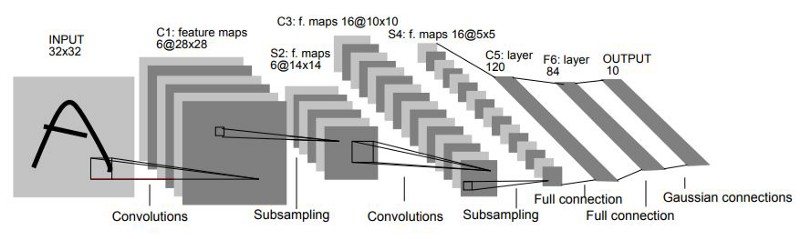
\includegraphics[width=\columnwidth]{images/lenet5.jpeg}
\captionof{figure}{Architecture de LeNet-5\cite{YannLeCunCNNs}}
\hfill\break

Nous observons deux couches de Convolution et deux couches de Pooling. On voit également le  
MLP composé d'une couche d'entrée, d'une couche cachée et d'une couche de sortie.

\subsection{Les couches de Convolution}
Nous verrons ici les calculs de propagation avant et de propagation arrière nécéssaires 
à l'entrainement des couches de convolution.\\

L'opération de convolution est définie par : 

\begin{align}
y[m,n] &= x[m,n] * h[m,n]\\
&=\sum^{\infty }_{j=-\infty}\sum^{\infty }_{i=-\infty}x[i,j]h[m-i,n-j]
\end{align}
Avec $x$ l'entrée, $y$ la sortie et $h$ le filtre.\\

Cependant, pour simplifier les calculs, nous éffectuerons des opérations de cross-corrélation, définis par : 

\begin{align}
    y[m,n] &= x[m,n] \star h[m,n]\\
    &=\sum^{\infty }_{j=-\infty}\sum^{\infty }_{i=-\infty}x[i,j]h[m+i,n+j]\\
    &= \sum^{\infty }_{j=-\infty}\sum^{\infty }_{i=-\infty}x[i,j] rot_{\ang{180}}\big[h[m-i,n-j]\big] \\
    &= x[m,n] * rot_{\ang{180}} \big[h[m,n]\big] 
\end{align}

Pour nos calculs, nous posons les termes suivant : \\

$l$ l'indice d'une couche\\
$y$ la sortie\\
$x$ l'entrée\\
$w$ le filtre (ou kernel) \\
$\sigma$ la fonction d'activation\\
$L$ la fonction coût\\
$m,n$ les indices des pixels de la sortie\\
$i,j$ les indices des pixels du filtre\\
$m',n'$ les indices des pixels de la dérivée de l'entrée\\
$i',j'$ les indices des pixels de la dérivée du filtre\\
$H,W$ la hauteur et la largeur de la sortie\\
$k$ la taille du filtre \\

Afin de simplifier les calculs théoriques, nous nous restreignons à une 
cross-corrélation sans padding et sur qu'un seul canal. \\

\subsubsection{Propagation Avant}

Une couche de convolution aura comme opération
en propagation avant : 

\begin{align}
y^{l} &= \sigma (y^{l-1})\star w^{l} \\
&=x^{l}\star w^{l} \\
y_{m,n}^{l} &= \sum_{j=0}^{k-1}\sum_{i=0}^{k-1}\sigma(y_{i,j}^{l-1}) \cdot w_{m+i,n+j}^{l}\\
&= \sum_{j=0}^{k-1}\sum_{i=0}^{k-1}\sigma(y_{m+i, n+j}^{l-1}) \cdot w_{i,j}^{l}
\end{align}

Cela génère des cartes de caractéristiques qui mettent en évidence certains 
motifs d’une image, aidant le MLP à la classifier. Le nombre de cartes 
correspond au nombre de filtres dans la couche. Par exemple, pour obtenir 6 cartes 
de caractéristiques, il faut utiliser 6 filtres différents.\\

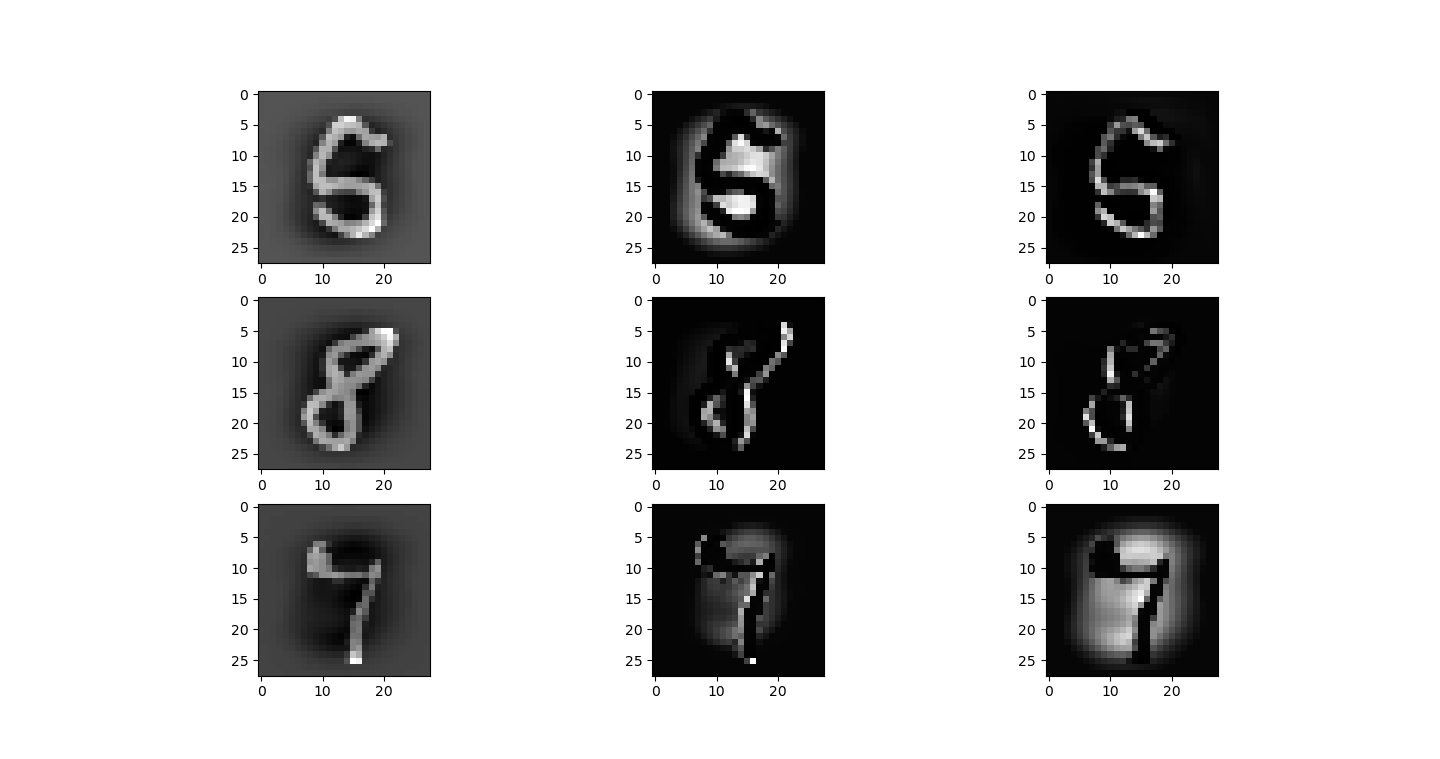
\includegraphics[width=\columnwidth]{images/featuremaps.png}
\captionof{figure}{Cartes de caractéristiques générées avec Melpy sur le dataset MNIST. 
Les entrées se situent dans la première colonne.}
\hfill\break

Sur la Figure 2, nous observons que certains pixels de l'image d'entrées sont
activés et d'autres non. On peut l'expliquer par le fait que les filtres 
vont être entrainés à activer uniquement certaines caractéristiques telles
que les bords verticaux, les bords horizontaux ou des formes plus complexes si nécessaire.\\


\subsubsection{Propagation Arrière}

En propagation arrière, nous aurons besoin des dérivées de la fonction coût $L$
par rapport à l'entrée $x^{l}$ et par rapport au filtre $w^{l}$.\\

Commençons par calculer $\frac{\partial L}{\partial w_{i',j'}^{l}}$ : 

{\scriptsize
\begin{align}
\frac{\partial L}{\partial w_{i',j'}^{l}} = \sum_{n=0}^{W-1}\sum_{m=0}^{H-1}\frac{\partial L}{\partial w_{i',j'}^{l}}\cdot\frac{\partial x_{m,n}^{l+1}}{\partial x_{m,n}^{l+1}}\\
= \sum_{n=0}^{W-1}\sum_{m=0}^{H-1}\frac{\partial L}{\partial x_{m,n}^{l+1}}\cdot\frac{\partial x_{m,n}^{l+1}}{\partial w_{i',j'}^{l}}
\end{align}}

On pose : 

$\frac{\partial{L}}{\partial{x_{m,n}^{l+1}}} = \delta^{l+1}_{m,n}$

{\scriptsize
\begin{align}
\implies \frac{\partial L}{\partial w_{i',j'}^{l}} &=  \sum_{n=0}^{W-1}\sum_{m=0}^{H-1}\delta^{l+1}_{m,n}\cdot\frac{\partial x_{m,n}^{l+1}}{\partial w_{i',j'}^{l}}\\
\frac{\partial x_{m,n}^{l+1}}{\partial w_{i',j'}^{l}}&= \frac{\partial}{\partial w_{i',j'}^{l}}\left(\sum_{j=0}^{W-1}\sum_{i=0}^{H-1}\sigma(x^{l}_{m+i, n+j}) \cdot w^{l}_{i,j}\right)\\
&= \frac{\partial}{\partial w^{l}_{i',j'}}\big (\sigma(x^{l}_{m+i', n+j'}) \cdot w^{l}_{i',j'}\big )\\
&= \sigma(x^{l}_{m+i', n+j'}) \cdot \frac{\partial}{\partial w^{l}_{i',j'}}\big (w^{l}_{i',j'}\big )\\
&= \sigma(x^{l}_{m+i',n+j'})\\
\implies \frac{\partial L}{\partial w_{i',j'}^{l}} &=  \sum_{n=0}^{W-1}\sum_{m=0}^{H-1}\delta^{l+1}_{m,n}\cdot\sigma(x^{l}_{m+i',n+j'})\\
&= \delta^{l+1}_{i',j'} \star \sigma(x^{l}_{i',j'})
\end{align}}

Calculons ensuite $\frac{\partial L}{\partial x^{l}_{m',n'}}$ : 

{\scriptsize
\begin{align}
\frac{\partial L}{\partial x^{l}_{m',n'}} &= \sum_{j=0}^{k-1}\sum_{i=0}^{k-1}\frac{\partial L}{\partial x_{m',n'}^{l}}\cdot\frac{\partial x_{m'-i,n'-j}^{l+1}}{\partial x_{m'-i,n'-j}^{l+1}}\\
&= \sum_{j=0}^{k-1}\sum_{i=0}^{k-1}\frac{\partial L}{\partial x_{m'-i,n'-j}^{l+1}}\cdot\frac{\partial x_{m'-i,n'-j}^{l+1}}{\partial x_{m',n'}^{l}}\\
&=   \sum_{j=0}^{k-1}\sum_{i=0}^{k-1}\delta^{l+1}_{m'-i,n'-j}\cdot\frac{\partial x_{m'-i,n'-j}^{l+1}}{\partial x_{m',n'}^{l}}\\
\begin{split}
    \frac{\partial x_{m'-i,n'-j}^{l+1}}{\partial x_{m',n'}^{l}} &= \frac{\partial}{\partial x^{l}_{m',n'}}\left( \sum_{j'=0}^{k-1}\sum_{i'=0}^{k-1}\right.  \\ 
    &  \biggl.\sigma(x^{l}_{m'-i+i',n'-j+j'})  \cdot w^{l}_{i',j'}  \bigg)
\end{split} \\
&= \frac{\partial}{\partial x^{l}_{m',n'}}\big(\sigma(x^{l}_{m',n'})\cdot w^{l}_{i,j}\big)\\
&= w^{l}_{i,j}\cdot \frac{\partial}{\partial x^{l}_{m',n'}}\big(\sigma(x^{l}_{m',n'})\big)\\
&= w^{l}_{i,j}\cdot \sigma'(x^{l}_{m',n'})\\
\implies \frac{\partial L}{\partial x^{l}_{m',n'}} &=  \sum_{j=0}^{k-1}\sum_{i=0}^{k-1}\delta^{l+1}_{m'-i,n'-j}\cdot w^{l}_{i,j}\cdot \sigma'(x^{l}_{m',n'})\\
&= \sum_{j=0}^{k-1}\sum_{i=0}^{k-1}\delta^{l+1}_{m'-i,n'-j}\cdot w^{l}_{i,j}\\
&= rot_{\ang{180}}\left \{ \sum_{j=0}^{k-1}\sum_{i=0}^{k-1}\delta^{l+1}_{m'+i,n'+j}\cdot w^{l}_{i,j} \right \} \\
& = \delta^{l+1}_{m',n'} \star rot_{\ang{180}}\{w^{l}_{m',n'}\}
\end{align}}

\textit{Lors du calcul de $\frac{\partial L}{\partial x^{l}_{m’,n’}}$, nous avons éffectué une convolution. 
Cela vient du fait que les éléments de la dérivée doivent être positionnés à l'emplacement des pixels 
ayant contribué aux erreurs correspondantes.}\\

Les dérivées calculées sont ensuite utilisées dans un algorithme de Descente de Gradient\cite{GradientDescent},
afin de mettre à jour le reste des paramètres du réseau.

\subsection{Les couches de Pooling}
Une couche de Pooling résume les informations d’une image en réduisant les pixels 
d’une fenêtre à une seule valeur représentative. Cette méthode, déjà présente en 1998 dans l'architecture de 
LeNet-5, réduit également le coût des calculs en temps et en mémoire. Nous étudierons 
ici l’une de ses variantes les plus courantes :  le Max Pooling. 

\subsubsection{Propagation Avant}

Le Pooling est une opération algorithmique donc nous n'aborderons pas
la formulation mathématique.\\

Deux paramètres influencent le Max Pooling : le \textit{stride} et 
la taille de la fenêtre (\textit{poolsize}). Le \textit{stride} détermine 
le nombre de pixels à sauter entre chaque position de la fenêtre.

Cette dernière de taille \textit{poolsize} parcourt les pixels en lignes 
et en colonnes, avec un pas de valeur \textit{stride}, pour produire une nouvelle 
image de taille $\lfloor \frac{Taille \ d’entr \acute{e}e - Poolsize}{Stride} + 1 \rfloor$. 
À chaque déplacement, elle sélectionne la valeur maximale de la fenêtre 
analysée, constituant un nouveau pixel de la sortie.\\

On peut visualiser l'opération de la manière suivante : \\

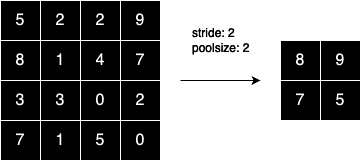
\includegraphics[width=\columnwidth]{images/forwardpooling.png}
\captionof{figure}{Exemple de la propagation avant d'un Max Pooling}
\hfill\break

Dans la Figure 3, nous voyons qu'un Max Pooling de \textit{poolsize} 2 et 
de \textit{stride} 2 a eu pour effet de diviser la taille de l'image par 2.\\

Sur une image réelle, l'opération donnerait le résultat suivant : \\

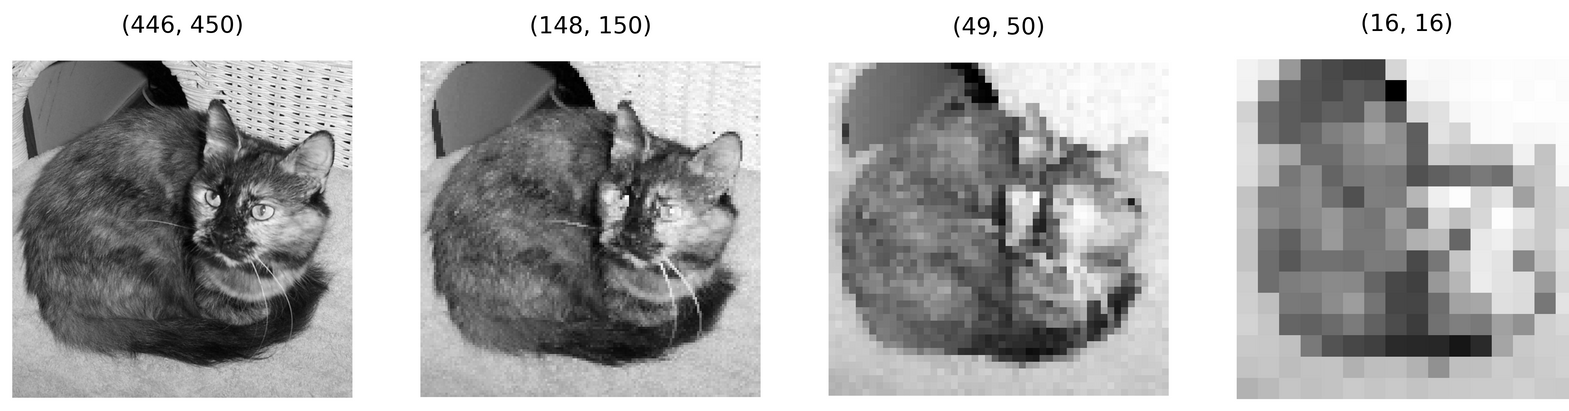
\includegraphics[width=\columnwidth]{images/maxpooling2.png}
\captionof{figure}{Exemple d'une opération de Max Pooling sur une image\cite{MaxPoolingImage2}}
\hfill\break

On observe ici une réduction de la taille de l’image tout en préservant ses 
informations essentielles.

\subsubsection{Propagation Arrière}

En propagation arrière, on redistribue les erreurs de la couche précédente, aux positions des
maxima utilisé en propagation avant. Les autres pixels sont quant à eux désactivés. \\

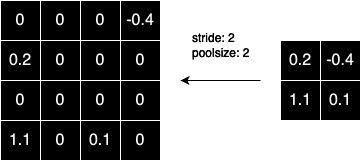
\includegraphics[width=\columnwidth]{images/backwardpooling.png}
\captionof{figure}{Exemple de la propagation arrière d'un Max Pooling}
\hfill\break

\end{multicols}
{\color{gray}\hrule}
\begin{center}
\section{Implémentation}
\textbf{Dans cette section, nous verrons l'implémentation des couches de 
pooling et de convolution à l'aide de NumPy.}
\bigskip
\end{center}
{\color{gray}\hrule}
\begin{multicols}{2}

Il existe diverses façons de réaliser un pooling et une convolution
en Python. La méthode la plus intuitive consiste à parcourir chaque pixel d’une
image avec des boucles, enregistrer les informations dans des listes, puis
effectuer les calculs élément par élément. Cependant, cette approche
s’avère très lente pour des opérations complexes sur plusieurs dimensions. \\

En effet, Python est un langage interprété, ce qui signifie que chaque
ligne de code est traduite en instructions machine à l’exécution.
Cela engendre une surcharge importante, surtout lorsque des boucles répétitives
traitent un grand volume de données. Ce manque d’efficacité devient rapidement problématique
avec des images de grande taille ou des ensembles volumineux. \\

Voici ci-dessous les résultats de calculs montrant la différence de temps entre une
méthode naïve et l’utilisation de NumPy pour effectuer un produit matriciel.\\

\renewcommand{\arraystretch}{1.5}

\scalebox{0.85}{
\begin{tabular}{l|c|r} 
\textbf{Dims de A} & \textbf{Dims de B} & \textbf{Rapport de temps}\\
$$ & $$ & $t_{1}$/$t_{2}$ \\
\hline
($10^{2}, 10^{1}$) & ($10^{1}, 10^{2}$) & $\frac{0.029}{0.00046}=63.04$\\
($10^{3}, 10^{2}$) & ($10^{2}, 10^{3}$) & $\frac{10.65}{0.07}=152.14$\\
($10^{3}, 10^{3}$) & ($10^{3}, 10^{3}$) & $\frac{124.64}{0.6}=207.73$\\
\end{tabular}
}\\

\captionof{table}{Comparaison des temps de calcul pour le produit matriciel entre les matrices A et B}

{\scriptsize
$t1$ le temps de calcul avec des boucles en secondes\\
$t2$ le temps de calcul avec NumPy en secondes\\
}

On vois dans Table 1 à la ligne 3, qu'il a fallu 2 minutes à la méthode naïve pour calculer 
le produit matriciel entre A et B contre 0,6 secondes pour NumPy.\\

L’utilisation de NumPy est donc à privilégier pour accélérer les calculs tensoriels. 
En effet, la bibliothèque est implémentée en C, ce qui permet d'effectuer des
opérations directement en langage machine. Le papier \textit{"The NumPy array: a structure for efficient numerical computation"}\cite{NumPyEfficiency}
explique bien son fonctionnement et le secret de cette rapidité.

\subsection{La méthode Im2Col}

Im2Col (image to column) est une méthode de vectorisation introduite en 2006 par 
trois chercheurs de l’Inria \cite{im2col}. Cette technique convertit les tenseurs 
d’images en matrices tout en les décomposant en fenêtres, ce qui simplifie les calculs 
de convolution et de pooling tout en s’intégrant naturellement avec NumPy. \\

L'opération se présente de la manière suivante :\\

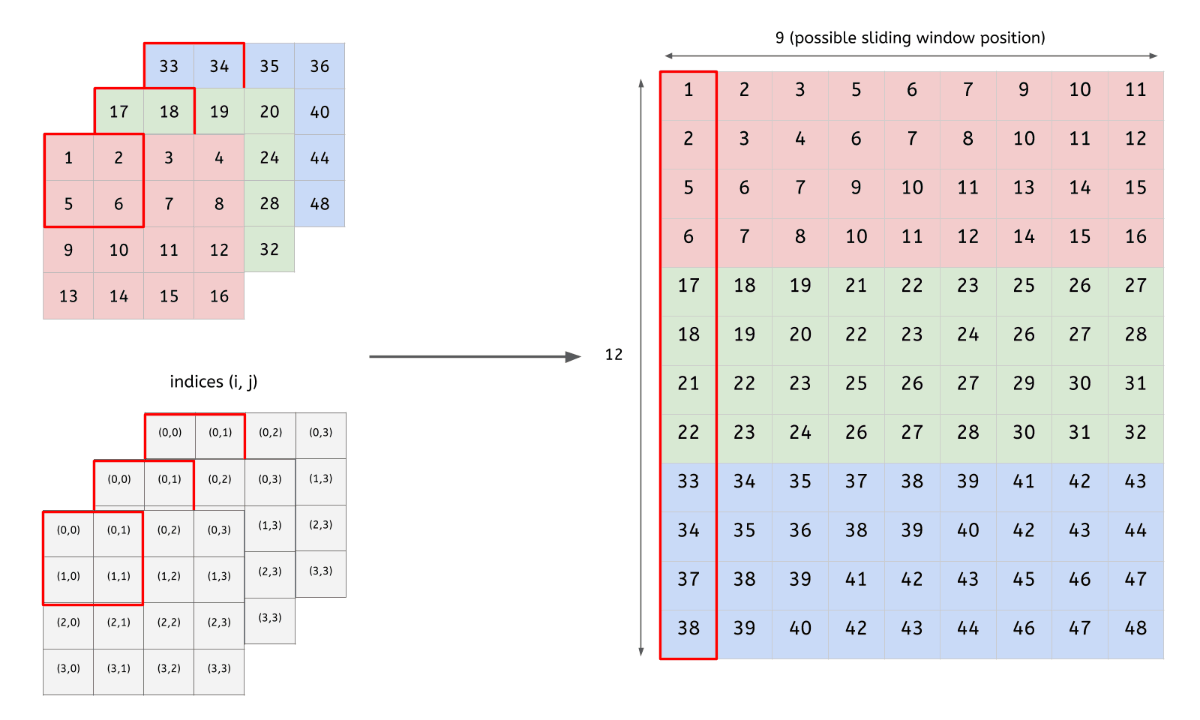
\includegraphics[width=\columnwidth]{images/im2col-1.png}
\captionof{figure}{Transformation en matrice d'une image RGB\cite{im2colImages}}
\hfill\break

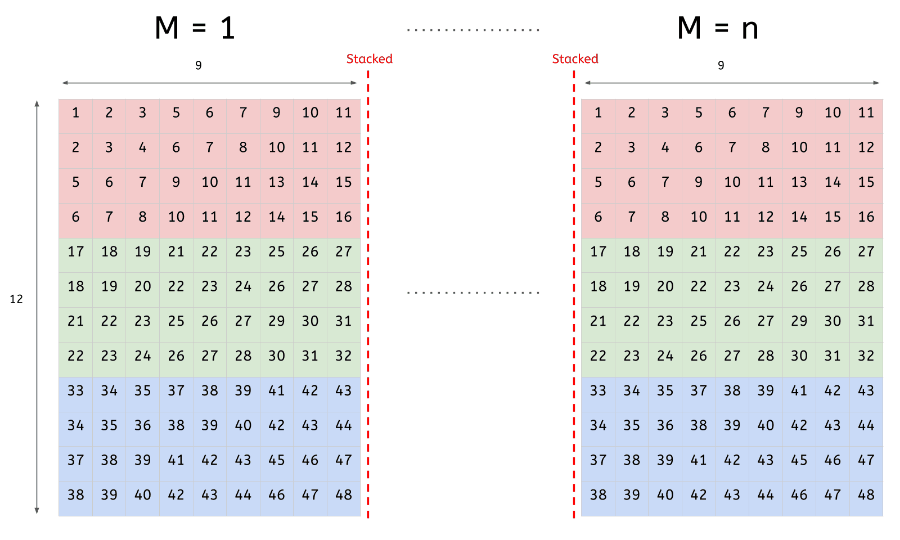
\includegraphics[width=\columnwidth]{images/im2col-2.png}
\captionof{figure}{Transformation en matrice de $n$ images RGB\cite{im2colImages}}
\hfill\break

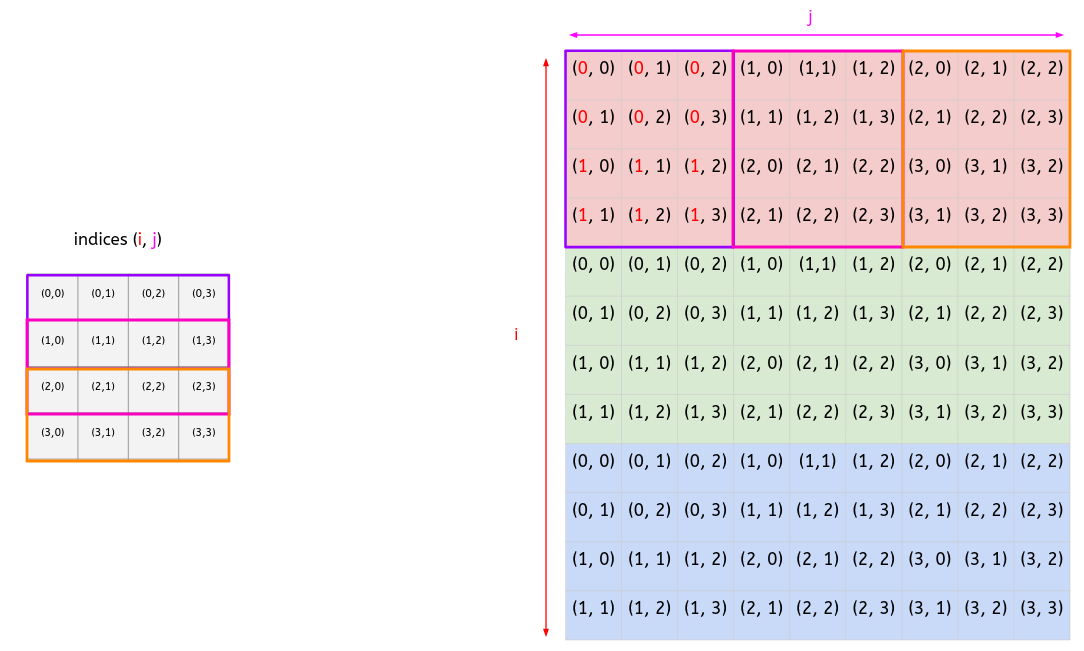
\includegraphics[width=\columnwidth]{images/im2col-3.png}
\captionof{figure}{Valeurs de la matrice remplacées par leurs indices dans l'image\cite{im2colImages}}
\hfill\break

Dans cet exemple, nous utilisons un $stride$ de 1 et une taille de fenêtre de valeur 2, sur des images de taille (4,4) en RGB. 
Comme illustré dans les Figures 6, 7 et 8, les canaux d’une image sont 
concaténés verticalement (de haut en bas), tandis que les fenêtres sont 
disposées horizontalement (de gauche à droite). De même, chaque image est 
concaténée horizontalement. \\

Nous avons, dans la Figure 8, remplacé les valeurs des pixels par leur position dans 
l’image, révélant ainsi des motifs récurrents. Ces motifs nous aideront à 
générer les indices $i$, $j$ et $k$ nécessaires pour construire la matrice à 
partir des positions des pixels. Examinons ces motifs en détail et 
modélisons-les mathématiquement. \\

Ici, le motif de l’indice $i$ au niveau 1 (zone violette dans la Figure 8) est $ (0,0,1,1) $. 
On remarque ensuite que les éléments sont additionnés par 1 au niveau 2 (zone rose dans la Figure 8) 
puis additionnés une nouvelle fois au niveau 3 (zone orange dans la Figure 8). Nous pouvons donc généraliser 
avec la formule suivante : \\

$ i_{m} = \{0_{0}+(m-1)\times stride,0_{1}+(m-1)\times stride,...,0_{k-1}+(m-1)\times stride, 1_{0}+(m-1)\times stride,1_{1}+(m-1)\times stride,...,1_{k-1}+(m-1)\times stride, (k-1)_{0}+(m-1)\times stride, (k-1)_{1}+(m-1)\times stride,..., (k-1)_{k-1}+(m-1)\times stride \}$,
où $m$ correspond au niveau, à partir de $m=1$ et $k$ la taille de la fenêtre. \\

Voici le code Python nécessaire pour générer les indices $i$ : \\

\begin{lstlisting}[language=Python]
import numpy as np

level1 = np.repeat(np.arange(window_shape), window_shape)
level1 = np.tile(level1, image_shape[1])

increment = stride * np.repeat(np.arange(output_height), output_width)

i = level1.reshape(-1, 1) + increment.reshape(1, -1)
\end{lstlisting} 
\hfill\break

Dans la ligne 3, \texttt{np.arrange(window\_shape)} génère une séquence d'entiers allant 
de 0 à \texttt{window\_shape-1} et \texttt{np.repeat(..., window\_shape)}
répète chaque élément de cette séquence un nombre de fois égal à \texttt{window\_shape}. \\

Dans la ligne 4, \texttt{np.tile(level1, image\_shape[1])} répète tout le tableau 
\texttt{level1} horizontalement un nombre de fois égal au nombre de canaux. \\

Dans la ligne 6, \texttt{np.arange(output\_height)} génère une séquence d’entiers allant
de 0 à \texttt{output\_height-1} et \texttt{np.repeat(..., output\_width)} répète chaque entier
de cette séquence un nombre de fois égal à \texttt{output\_width}. Ensuite, le résultat
est multiplié par le $stride$. \\

Dans la ligne 8, \texttt{level1.reshape(-1, 1)} transforme le tableau level1 en un
vecteur colonne. De même, \texttt{increment.reshape(1, -1)} transforme le tableau \texttt{increment} en un vecteur 
ligne. L’addition entre ces deux matrices suit les règles de broadcasting de NumPy\cite{NumPyEfficiency}, 
combinant chaque élément de \texttt{level1} avec chaque élément de increment pour produire une matrice
contenant l'ensemble des indices $i$. \\

Concernant l’indice $j$, les motifs observés sont : 
$j_{1,2,3} = \{(0,1,0,1),(1,2,1,2),(2,3,2,3)\}$. On voit qu'à chaque déplacement 
de la fenêtre, les indices $j$ sont additionnés par 1 à partir de $j_{1}$. On peut donc généraliser
de la manière suivante : \\

$j_{n} = \{0_{0}+(n-1) \times stride,1_{0}+(n-1)\times stride,...,(k-1)_{0}+(n-1)\times stride,...,0_{k-1}+(n-1)\times stride,1_{k-1}+(n-1)\times stride,...,(k-1)_{k-1}+(n-1)\times stride\}$\\
où $n$ correspond au glissement, à partir de $n=1$ et $k$ la taille de la fenêtre. \\

Voici le code Python nécessaire pour générer les indices $j$ : \\

\begin{lstlisting}[language=Python]
import numpy as np

slide1 = np.tile(np.arange(window_shape), window_shape * image_shape[1])
increment = stride * np.tile(np.arange(output_width), output_height)

j = slide1.reshape(-1, 1) + increment.reshape(1, -1)
\end{lstlisting}
\hfill\break

Dans la ligne 3, \texttt{np.arange(window\_shape)} génère une séquence d’entiers allant
de 0 à \texttt{window\_shape-1} et \texttt{np.repeat(..., window\_shape)} répète chaque élément
de cette séquence un nombre de fois égal à \texttt{window\_shape}. \\

Dans la ligne 4, \texttt{np.tile(level1, image\_shape[1])} répète tout le tableau
level1 horizontalement un nombre de fois égal au nombre de canaux. \\

Dans la ligne 6, \texttt{np.arange(output\_height}) génère une séquence d’entiers allant
de 0 à \texttt{output\_height-1} et \texttt{ np.repeat(..., output\_width)} répète chaque entier
de cette séquence un nombre de fois égal à \texttt{output\_width}. Ensuite, le résultat
est multiplié par le $stride$. \\

Dans la ligne 8, \texttt{slide1.reshape(-1, 1)} transforme le tableau \texttt{slide1} en un
vecteur colonne. De même, \texttt{increment.reshape(1, -1)} transforme le tableau \texttt{increment} en un vecteur
ligne. L’addition entre ces deux matrices suit, encore une fois, les règles de broadcasting de NumPy\cite{NumPyEfficiency},
combinant chaque élément de slide1 avec chaque élément de increment pour produire
une matrice contenant l’ensemble des indices $j$. \\

Concernant l’indice des canaux  $k$, il suffit de répéter les indices des canaux pour 
chaque pixel dans une fenêtre. \\

Voici le code Python nécessaire pour générer les indices $k$ : \\

\begin{lstlisting}[language=Python]
import numpy as np

k = np.repeat(np.arange(image_shape[1]), window_shape * window_shape).reshape(-1, 1)  
\end{lstlisting}
\hfill\break

Dans cette ligne, \texttt{np.arange(image\_shape[1])} génère une séquence d’entiers allant
de 0 au nombre de canaux de l’image. Ensuite, \texttt{np.repeat(..., window\_shape * window\_shape)} répète chaque entier de 
cette séquence un nombre de fois égal à \texttt{window\_shape * window\_shape}, c’est-à-dire le nombre de pixels dans une fenêtre.
Enfin, \texttt{.reshape(-1, 1)} transforme le tableau résultant en un vecteur colonne, contenant l'ensemble
des indices $k$. \\

Maintenant que nous avons les indices, il reste à générer la matrice 
correspondant au jeu de données :\\

\begin{lstlisting}[language=Python]
import numpy as np

k, i, j = get_indices(images.shape, window_shape, stride)
columns = np.concatenate(images[:, k, i, j], axis=-1)
\end{lstlisting}

Dans ce code, chaque image est vectorisée puis concaténée avec les précédentes. 
À la fin, nous obtenons des colonnes de matrices correspondant à chacune d'entre elles. \\

L'opération inverse (Col2Im) est également possible en replaçant chaque pixel 
à sa position initiale :

\begin{lstlisting}[language=Python]
import numpy as np

images = np.zeros(image_shape)
k, i, j = get_indices(image_shape, window_shape, stride)
cols_reshaped = np.array(np.hsplit(columns, image_shape[0]))
np.add.at(images, (slice(None), k, i, j), cols_reshaped)
\end{lstlisting}

Dans le cas où le $stride$ crée des fenêtres qui se superposent,
les pixels sont additionnés aux positions concernées (voir Figure 9). Cela n'aura pas 
d'effets négatifs dans nos calculs étant donné que cela réspecte leur 
contribution.\\

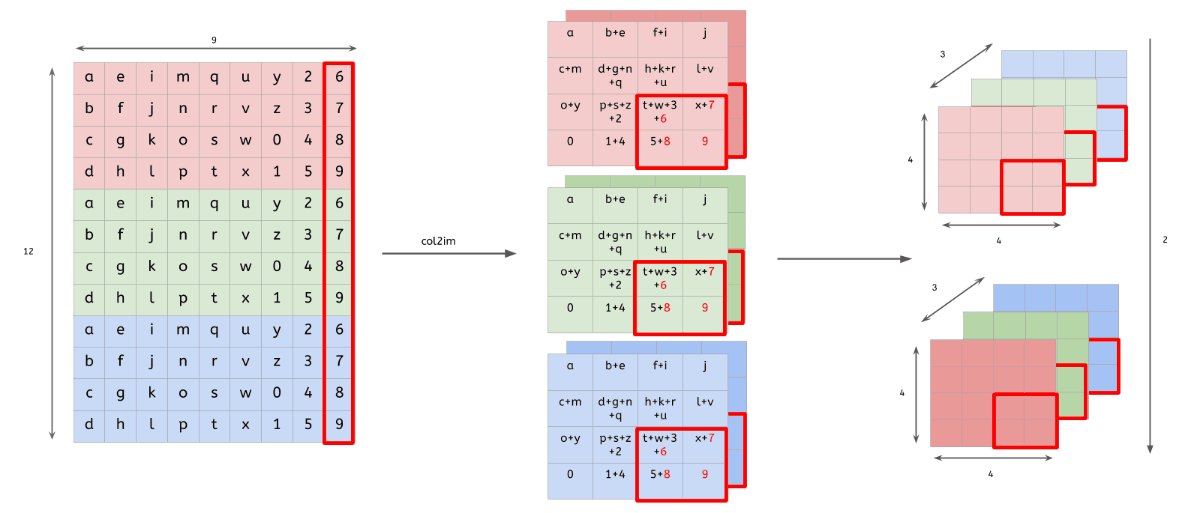
\includegraphics[width=\columnwidth]{images/im2col-4.png}
\captionof{figure}{Opération Col2Im\cite{im2colImages}}
\hfill\break

L'ensemble du code de la méthode Im2col se trouve dans le repo de Melpy,
à l'adresse suivante : \url{https://github.com/lennymalard/melpy-project/blob/main/melpy/im2col.py}

\subsection{Les couches de convolution}

Les couches $convolution2D$ héritent de la superclasse $Layer$ 
de Melpy, ce qui leur impose l’utilisation des méthodes 
\textbf{forward()} et \textbf{backward()} pour effectuer 
respectivement les propagations avant et arrière.\\

Voici, dans un premier temps, le code de la propagation avant :\\

\begin{lstlisting}[language=Python]
def forward(self):
    self.input_padded = self.explicit_padding()

    self.input_cols = im2col(self.input_padded, self.kernel_size, self.stride)
    self.filter_cols = self.weights.reshape(self.out_channels, -1)

    output_height, output_width = self.get_output_size(self.inputs.shape[2], self.inputs.shape[3])

    self.output_cols = self.filter_cols @ self.input_cols

    self.outputs = np.array(np.hsplit(self.output_cols, self.inputs.shape[0])).reshape(
        (self.input_padded.shape[0], self.out_channels, output_height, output_width)
    )

    if self.biases is not None:
        self.outputs += self.biases

    return self.outputs
\end{lstlisting}
\hfill\break

Les images d’entrée sont d’abord paddées via \texttt{self.explicit\_padding()} pour ajuster leurs dimensions, 
puis converties en colonnes avec \texttt{im2col()}. Les poids de la couche sont également aplatis en une 
matrice pour pouvoir effectuer un produit matriciel avec les colonnes d’images. Les dimensions de sortie sont 
calculées avec \texttt{self.get\_output\_size()}, et la convolution est réalisée en multipliant les colonnes des images 
par les filtres aplatis. Les résultats sont réassemblés en images, ajustés si des biais sont 
présents, puis retournés comme résultats finaux de la couche pour être propagés en avant.\\

Voici maintenant le code de la propagation arrière : \\

\begin{lstlisting}[language=Python]
def backward(self, dX):
    self.dY = dX

    flipped_filters = self.weights[:, :, ::-1, ::-1]
    flipped_filters_cols = flipped_filters.reshape(self.out_channels, -1)

    self.dY_reshaped = self.dY.reshape(self.dY.shape[0] * self.dY.shape[1], self.dY.shape[2] * self.dY.shape[3])
    self.dY_reshaped = np.array(np.vsplit(self.dY_reshaped, self.inputs.shape[0]))
    self.dY_reshaped = np.concatenate(self.dY_reshaped, axis=-1)

    self.dX_cols = flipped_filters_cols.T @ self.dY_reshaped
    self.dW_cols = self.dY_reshaped @ self.input_cols.T

    self.dX_padded = col2im(self.dX_cols, self.input_padded.shape, self.kernel_size, self.stride)

    if self.padding == "same":
        (pad_top, pad_bottom, pad_left, pad_right) = self.calculate_padding()
        self.dX = self.dX_padded[:, :, pad_top:-pad_bottom, pad_left:-pad_right]
    else:
        self.dX = self.dX_padded

    self.dW = self.dW_cols.reshape((self.dW_cols.shape[0], self.in_channels, self.kernel_size, self.kernel_size))

    if self.biases is not None:
        self.dB = np.sum(self.dY, axis=(0, 2, 3), keepdims=True)

    return self.dX
\end{lstlisting}
\hfill\break

Les gradients de sortie \texttt{dX} sont assignés à \texttt{self.dY}, et les filtres sont 
retournés de \ang{180} puis aplatis en colonnes pour les calculs. Les gradients \texttt{self.dY} 
sont convertis en colonnes, et les gradients des entrées \texttt{self.dX} sont calculés 
via un produit matriciel entre les colonnes des filtres retournés et $dY$. 
Les gradients des poids \texttt{self.dW} sont quant à eux obtenus par multiplication entre $dY$ et 
les colonnes d’entrée transposées. Les gradients des biais \texttt{self.dB}, si présents, sont calculés par une somme. 
Les gradients d’entrée sont reconstitués avec \texttt{col2im()} et ajustés pour retirer le padding si nécessaire. 
Finalement, les gradients \texttt{self.dX} sont retournés pour poursuivre la propagation arrière. \\

L'ensemble du code lié aux couches de convolution se trouvent dans le repo de Melpy, à l'adresse suivante : \url{https://github.com/lennymalard/melpy-project/blob/main/melpy/layers.py}

\subsection{Les couches de pooling}

Les couches $pooling2D$ héritent également de la superclasse $Layer$ 
de Melpy, leur imposant les mêmes contraintes que $convolution2D$.\\

Voici donc le code de la propagation avant : \\

\begin{lstlisting}[language=Python]
def forward(self):
    output_height = int((self.inputs.shape[2] - self.pool_size + self.stride) // self.stride)
    output_width = int((self.inputs.shape[3] - self.pool_size + self.stride) // self.stride)

    output_shape = (self.inputs.shape[0], self.inputs.shape[1], output_height, output_width)

    self.input_cols = im2col(self.inputs, self.pool_size, self.stride)
    self.input_cols_reshaped = np.array(np.hsplit(np.array(np.hsplit(self.input_cols, self.inputs.shape[0])), self.inputs.shape[1]))

    self.maxima = np.max(self.input_cols_reshaped, axis=2)
    self.maxima_reshaped = self.maxima.reshape(self.inputs.shape[1], -1)

    self.outputs = col2im(self.maxima_reshaped, output_shape, 1, 1)

    return self.outputs
\end{lstlisting}
\hfill\break

Les dimensions de sortie sont d’abord calculées, en fonction des dimensions d’entrée, 
de la taille de la fenêtre de pooling, et du $stride$. Les entrées sont ensuite 
transformées en colonnes à l’aide de \texttt{im2col()}. Les colonnes sont restructurées pour 
correspondre aux canaux et échantillons, puis l’opération \texttt{np.max()}
extrait les maxima de chaque fenêtre. Ces valeurs maximales sont réorganisées et 
reconstruites en utilisant \texttt{col2im()} pour former les sorties finales.
Ces sorties sont finalement retournées pour poursuivre la propagation avant.\\

Voici maintenant le code de la propagation arrière : \\

\begin{lstlisting}[language=Python]
def backward(self, dX):
    self.dY = dX
    self.dX = np.zeros_like(self.inputs)

    self.dY_cols = im2col(self.dY, 1, 1)
    self.dY_cols_reshaped = np.array(np.hsplit(np.array(np.hsplit(self.dY_cols, self.dY.shape[0])), self.dY.shape[1])).transpose(0, 1, 3, 2)

    self.input_cols = im2col(self.inputs, self.pool_size, self.stride)
    self.input_cols_reshaped = np.array(np.hsplit(np.array(np.hsplit(self.input_cols, self.inputs.shape[0])), self.inputs.shape[1])).transpose(0, 1, 3, 2)

    self.output_cols = im2col(self.outputs, 1, 1)
    self.output_cols_reshaped = np.array(np.hsplit(np.array(np.hsplit(self.output_cols, self.inputs.shape[0])), self.inputs.shape[1])).transpose(0, 1, 3, 2)

    self.mask = np.array(self.input_cols_reshaped == self.output_cols_reshaped, dtype=np.uint64)

    self.dX_cols = np.concatenate(np.concatenate(np.array(self.mask * self.dY_cols_reshaped).transpose(0, 1, 3, 2), axis=1), axis=1)
    self.dX = col2im(self.dX_cols, self.inputs.shape, self.pool_size, self.stride)

    return self.dX
\end{lstlisting}
\hfill\break

Les gradients reçus \texttt{dX} sont sauvegardés dans \texttt{self.dY}, puis 
transformés en colonnes avec \texttt{im2col()}. Les entrées 
originales et les sorties de la propagation avant sont également converties en colonnes et 
restructurées. Un masque binaire identifiant les maxima des fenêtres de pooling est créé 
pour ne transmettre que les gradients associés à ces maxima. Les gradients modifiés sont 
réassemblés en une forme plate, puis reconstruits avec \texttt{col2im()} pour correspondre 
aux dimensions des entrées. Enfin, les gradients des entrées reconstitués \texttt{self.dX}
sont retournés pour continuer la propagation arrière. \\

L'ensemble du code lié aux couches de pooling se trouvent dans le repo de Melpy, à l'adresse suivante : \url{https://github.com/lennymalard/melpy-project/blob/main/melpy/layers.py}

\end{multicols}



{\color{gray}\hrule}
\begin{center}
\section{Expérimentations}
\textbf{Dans cette section, nous verrons les expérimentations éffectuées et discuterons de leurs résulats.}
\bigskip
\end{center}
{\color{gray}\hrule}
\begin{multicols}{2}

Pour évaluer la justesse et l’efficacité de l’implémentation, il a fallu entraîner 
des architectures, ajuster leurs hyperparamètres, puis comparer les résultats obtenus avec 
ceux de Keras sur les mêmes architectures. \\

Le jeu de données MNIST a été choisi pour le premier test. Composé de 
60 000 images de chiffres manuscrits (de 0 à 9), il est l’un des jeux de données 
les plus connus pour les tâches de classification d’images. Chaque image mesure 
28x28 pixels et est en niveaux de gris. Ce jeu de données est particulièrement
populaire car il est simple à traiter et offre une grande qualité et quantité 
d’exemples, ce qui en fait une référence pour les premières expérimentations en 
apprentissage profond. \\

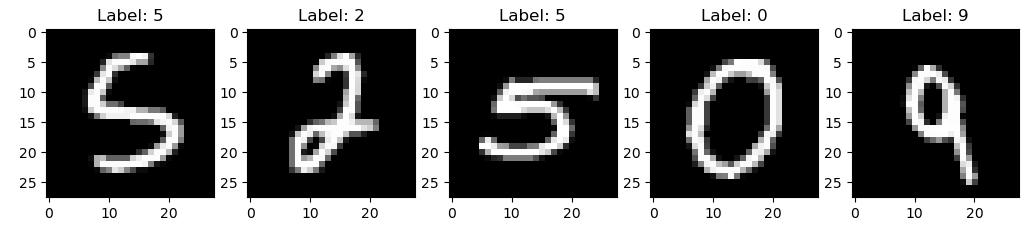
\includegraphics[width=\columnwidth]{images/mnist_samples.png}
\captionof{figure}{Exemples d'images provenant du jeu de données MNIST}
\hfill\break

Cependant, afin d’augmenter la complexité des expérimentations, le jeu de données CIFAR-10\cite{CIFAR10} a également 
été utilisé. Il contient 60 000 images réparties en 10 classes (avions, voitures, oiseaux, chats, cerfs, 
chiens, grenouilles, chevaux, bateaux et camions). Les images sont des photographies sous échantillonnées, qui mesurent 32x32 pixels et qui sont en couleur 
(format RGB), ce qui les rend plus complexes à traiter que celles de MNIST. La diversité des classes et le manque de corrélation 
entre elles ajoutent également de la complexité à ce jeu de données. En ce qui concerne la qualité de ces dernières,
elle est comparable à celle de MNIST. \\

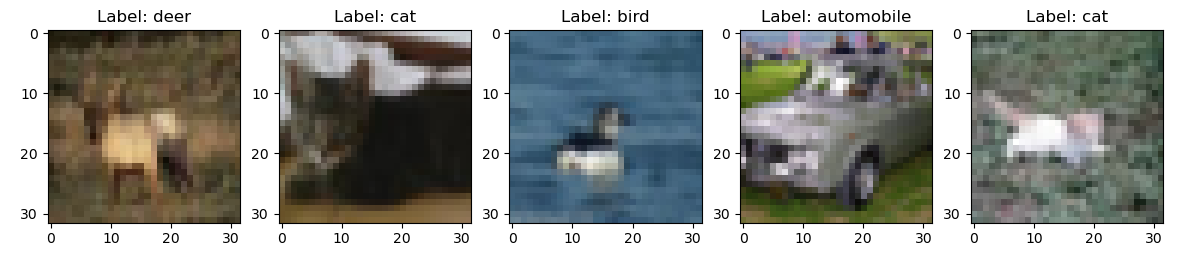
\includegraphics[width=\columnwidth]{images/cifar10_samples.png}
\captionof{figure}{Exemples d'images provenant du jeu de données CIFAR-10}
\hfill\break

\subsection{Méthode}

Le protocole expérimental est le suivant :  \\


\textbf{Pré-traitement des données} Les données sont pré-traitées 
pour être compatibles avec les modèles.\\

\textbf{Création et évaluation d’architectures avec Melpy} Des architectures sont créées 
et entraînées avec différents hyperparamètres pour identifier celle qui offre 
la meilleure généralisation.\\

\textbf{Création et entraînement des architectures avec Keras} L'architecture
sélectionnée est ensuite entraînée avec Keras de manière similaire.


\textbf{Comparaison des métriques finales} On compare les métriques finales d'une bibliothèque
avec celles de l'autres. \\

L’entraînement a été effectué sur un processeur Intel i5-12600K avec 32 Go de RAM. Il est important de 
noter que les temps de calcul ont pu être influencés par des processus externes indésirables. Concernant 
la métrique utilisée, seul le coût de l’architecture au fil des époques a été présenté, car il reflète 
très bien les performances d’un modèle. \\


\subsection{Résultats et discussion}

\subsubsection{Pré-traitement des données}

Afin d’éviter des problèmes tels que \textit{Dead ReLU}, l’explosion des gradients 
ou encore la disparition des gradients, il est nécessaire de mettre les images à l’échelle.\\

Pour ce faire, nous commençons par normaliser les données, en les mettant sur une 
échelle allant de 0 à 1, puis nous les standardisons.\\

Enfin, les étiquettes doivent être encodées. Pour cela, nous utilisons l’encodeur One-Hot.\\

\subsubsection{Sélection du modèle}

\textbf{MNIST} \\

L'architecture sélectionnée pour MNIST est la suivante : \\

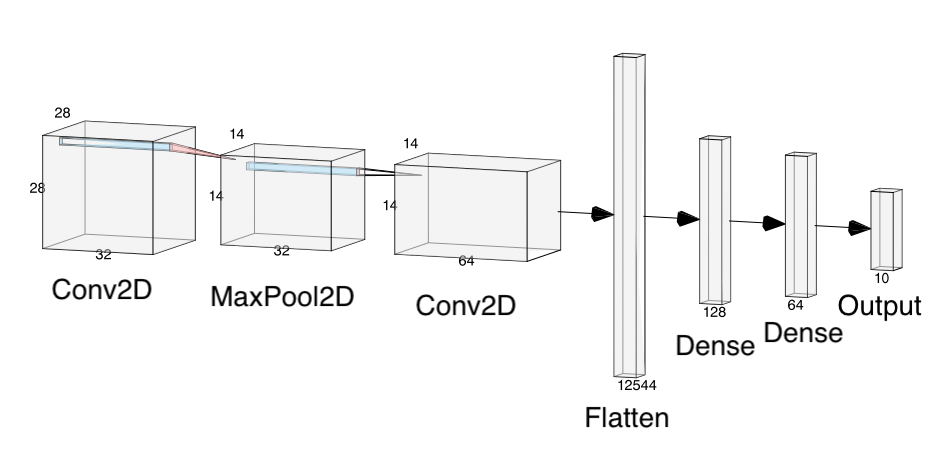
\includegraphics[width=\columnwidth]{images/mnist_nn.png}
\captionof{figure}{Réseau de neurones sélectionné pour MNIST}
\hfill\break

Comme illustré dans la Figure 10, le réseau de neurones commence par une couche de convolution qui 
génère 16 cartes de caractéristiques, suivie d’une couche de pooling qui réduit leur taille de moitié.
Ensuite, une seconde couche de convolution produit 32 cartes de caractéristiques, ensuite aplaties pour alimenter 
un MLP ayant une couche cachée composée de 128 neurones. \\

La couche cachée utilise la fonction d’activation Leaky ReLU, tandis que la sortie 
applique une fonction Softmax. Pour optimiser l'architecture, l’algorithme Adaptive Momentum (Adam) a été utilisé pour minimiser 
la fonction de coût d’entropie croisée catégorielle (Categorical Cross-Entropy). \\

Le choix a été fait sur les 5 entrainements suivants : \\

\scalebox{0.55}{
\begin{tabular}{l|c c c c c c c|}
    \cline{2-8}
                                   & $P$                  & $\Delta$                          & $e$           &$t/e$              & Lot     & $\gamma$             & $t$              \\
    \hline
    \multicolumn{1}{|l|}{$1$}      & 15 840               & $1C_{w, b}+2D_{w,b} = 3$     & 15            & 32sec             & 256     & $1^{-4}$             &08min 01sec           \\             
    \multicolumn{1}{|l|}{$2$}      & 201 226              & $1C_{w, b}+2D_{w,b} = 3$     & 15            & 02min 23sec       & 256     & $1^{-4}$             &35min 58sec           \\ 
    \multicolumn{1}{|l|}{$3$}      & 806 394              & $2C_{w, b}+2D_{w,b} = 4$     & 15            & 01min 53sec       & 256     & $1^{-4}$             &28min 22sec           \\ 
    \multicolumn{1}{|l|}{$4$}      & 1 624 842            & $2C_{w, b}+4D_{w,b} = 6$     & 10            & 04min 42sec       & 256     & $1^{-4}$             &47min 03sec \\
    \multicolumn{1}{|l|}{$5$}      & 1 615 466            & $2C_{w, b}+2D_{w,b} = 4$     & 10            & 04min 40sec       & 256     & $1^{-4}$             &46min 49sec  \\
    \hline
\end{tabular}}
\captionof{table}{Entrainements éffectués sur MNIST avec Melpy} \\

{\scriptsize
$P$ étant le nombre de paramètres dans l'architecture\\

$\Delta$ étant la prodondeur de l'architecture avec $C$ une couche de convolution, D une couche entièrement connectée, $w$ l'utilisation de poids et $b$ l'utilisation de biais \\

$e$ étant le nombre d'époques passés pour entrainer l'architecture \\

$Lot$ étant le nombre d'entrées entrainées sur une passe avant et arrière \\

$\gamma$ étant le taux d'apprentissage utilisé dans l'algorithme d'optimisation \\

$t$ étant le temps qu'il a fallu pour entrainer l'architecture \\

$t/e$ étant le temps passé en moyenne sur une époque \\
} \\
\textit{La taille des lots et le taux d’apprentissage restent ici inchangés, car ils se sont révélés significativement plus stables 
que d'autres configurations testées, n'apportant pas d’informations pertinentes sur les entrainements.} \\


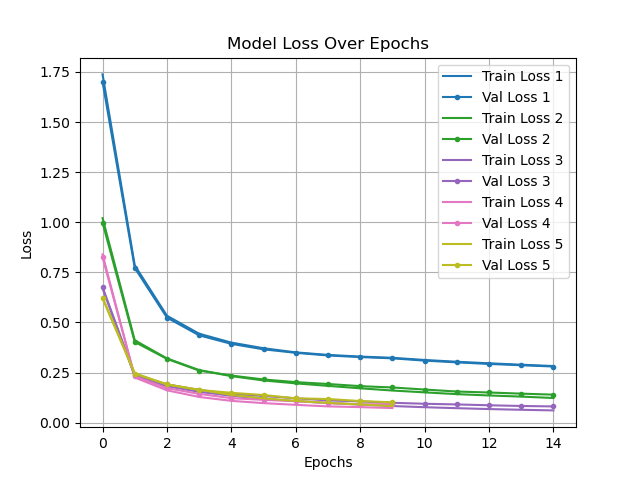
\includegraphics[width=\columnwidth]{images/mnist_losses.png}
\captionof{figure}{Le coût de l'architecture au fil des époques}
\hfill\break

Comme l’illustre la Figure 13, les modèles 3, 4 et 5 présentent des performances similaires. 
Cependant, le modèle 3 est sélectionné en raison de sa rapidité d’exécution sur une 
époque (voir Table 2). \\

En dehors de la sélection d’un modèle à comparer avec Keras, nous pouvons relever les informations suivantes concernant les différents entrainements :
\begin{itemize}
\item \textbf{Nombre de paramètres} : Le nombre de paramètres influence significativement le temps nécessaire pour réaliser une époque.
\item \textbf{Complexité du modèle} : Les modèles plus complexes tendent à mieux détecter les motifs. Cependant, cette complexité devient moins efficace 
lorsque le nombre de neurones ou la profondeur de l’architecture devient excessif.
\end{itemize} 
\hfill\break

\textbf{CIFAR-10} \\

L'architecture sélectionnée pour CIFAR-10 est la suivante : \\

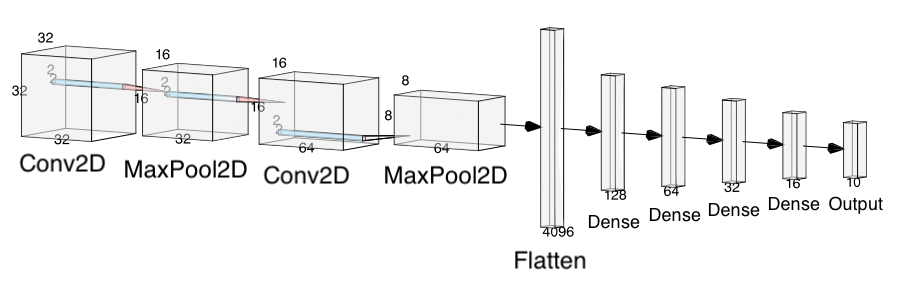
\includegraphics[width=\columnwidth]{images/cifar10_nn.png}
\captionof{figure}{Réseau de neurones sélectionné pour CIFAR-10}
\hfill\break


Comme illustré dans la Figure 14, le réseau de neurones débute par une couche de convolution générant 32 cartes de caractéristiques, suivie d’une couche de pooling réduisant leur taille de moitié. 
Cette opération est répétée une seconde fois, avec comme seule différence la couche de convolution produisant cette fois 64 cartes de caractéristiques.
Celles-ci sont ensuite aplaties pour alimenter un MLP constitué de 4 couches cachées contenant respectivement 128, 64, 32 et 16 neurones chacune. \\

Les couches cachées utilisent la fonction d’activation Leaky ReLU, tandis que la sortie 
applique une fonction Softmax. Pour optimiser l'architecture, l’algorithme Adam a été utilisé pour minimiser 
la fonction de coût d’entropie croisée catégorielle. \\

Le choix a été fait sur les 6 entrainements suivants : \\

\scalebox{0.515}{
\begin{tabular}{l|c c c c c c c|}
    \cline{2-8}
                                   & $P$                  & $\Delta$                     & $e$           &$t/e$        & Lot     & $\gamma$             & $t$              \\
    \hline
    \multicolumn{1}{|l|}{$1$}      & 1 056 376            & $4C_{w}+2D_{w,b} = 6$        & 20            & 09min 50sec & 128     & $5^{-5}$             &03h 16min 59sec           \\
    \multicolumn{1}{|l|}{$2$}      & 2 107 146            & $2C_{w}+2D_{w,b} = 4$        & 20            & 17min 24sec & 128     & $1^{-5}$             &05h 48min 14sec           \\
    \multicolumn{1}{|l|}{$3$}      & 2 107 146            & $2C_{w}+2D_{w,b} = 4$        & 35            & 15min 38sec & 128     & $5^{-5}$             &09h 07min 21sec           \\
    \multicolumn{1}{|l|}{$4$}      & 2 107 146            & $2C_{w}+2D_{w,b} = 4$        & 50            & 08min 12sec & 256     & $5^{-5}$             &06h 50min 36sec          \\
    \multicolumn{1}{|l|}{$5$}      & 2 117 866            & $2C_{w}+2D_{w,b} = 4$        & 100           & 10min 27sec & 128     & $5^{-5}$             &17h 26min 00sec           \\
    \multicolumn{1}{|l|}{$6$}      & 8 398 698            & $2C_{w,b}+2D_{w,b} = 4$      & 50            & 08min 34sec & 64      & $5^{-6}$             &07h 08min 29sec           \\
    \multicolumn{1}{|l|}{$7$}      & 544 122              & $2C_{w,b}+5D_{w,b} = 7$      & 50            & 05min 53sec & 64      & $5^{-5}$             &04h 54min 52sec           \\
    \multicolumn{1}{|l|}{$8$}      & 8 408 442            & $2C_{w,b}+5D_{w,b} = 7$      & 50            & 10min 26sec & 64      & $5^{-5}$             &08h 42min 17sec           \\
    \hline
\end{tabular}}
\captionof{table}{Entrainements éffectués sur CIFAR-10 avec Melpy} \\

{\scriptsize
$P$ étant le nombre de paramètres dans l'architecture\\

$\Delta$ étant la prodondeur de l'architecture avec $C$ une couche de convolution, D une couche entièrement connectée, $w$ l'utilisation de poids et $b$ l'utilisation de biais \\

$e$ étant le nombre d'époques passés pour entrainer l'architecture \\

$Lot$ étant le nombre d'entrées entrainées sur une passe avant et arrière \\

$\gamma$ étant le taux d'apprentissage utilisé dans l'algorithme d'optimisation \\

$t$ étant le temps qu'il a fallu pour entrainer l'architecture \\

$t/e$ étant le temps passé en moyenne sur une époque \\
} \\

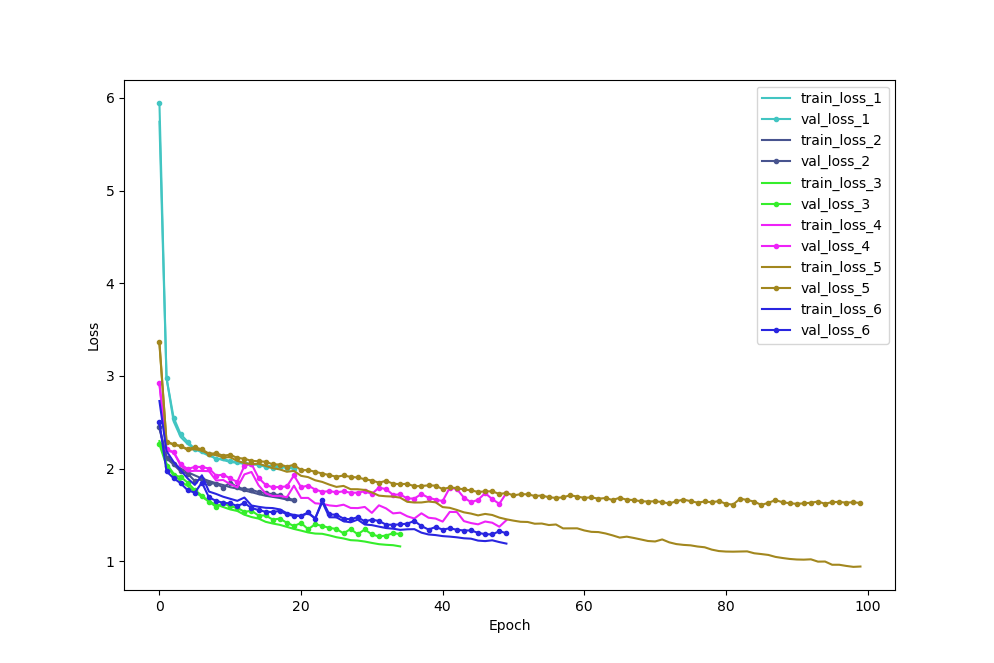
\includegraphics[width=\columnwidth]{images/cifar_10_losses.png}
\captionof{figure}{Le coût de l'architecture au fil des époques}
\hfill\break

Comme le montre la Figure 15, les modèles 3, 7 et 8 se démarquent comme 
les plus performants. Parmi eux, c'est bien le modèle 7 qui a été retenu. Ce choix repose sur un 
compromis entre la qualité de sa généralisation, son temps d’entraînement réduit et 
son efficacité dès le début de ce dernier. \\

À l'instar des entrainements sur MNIST, nous pouvons relever les informations suivantes à partir de l'ensemble des entrainements sélectionnés pour CIFAR-10 :  
\begin{itemize}
    \item \textbf{Taille des lots} : Elle influence de manière significative le temps de calcul par époque ainsi que le nombre d’itérations nécessaires pour atteindre 
    la convergence.
    \item \textbf{Capacité de généralisation} : La taille des lots influence également la capacité du modèle à bien généraliser sur des données non vues, à condition que le modèle ne soit pas trop complexe.
    \item \textbf{Couches de pooling} : L’intégration de couches de pooling à des positions intéressantes dans l’architecture peut compenser le temps de calcul, 
    bien que cela se fasse au détriment de la quantité d’informations utilisé pour l’apprentissage.
\end{itemize}
\hfill\break


\subsubsection{Comparaison des résultats}

Afin d’évaluer les performances de Melpy dans l’utilisation des CNNs, nous comparons cette bibliothèque avec Keras, une autre bibliothèque de deep learning, reconnue pour la simplicité de son utilisation. \\

Pour ce faire, ce sont les architectures sélectionnées plus tôt qui serviront de référence.\\

Observons les différences dans le calcul du coût pour chaque jeu de données : \\

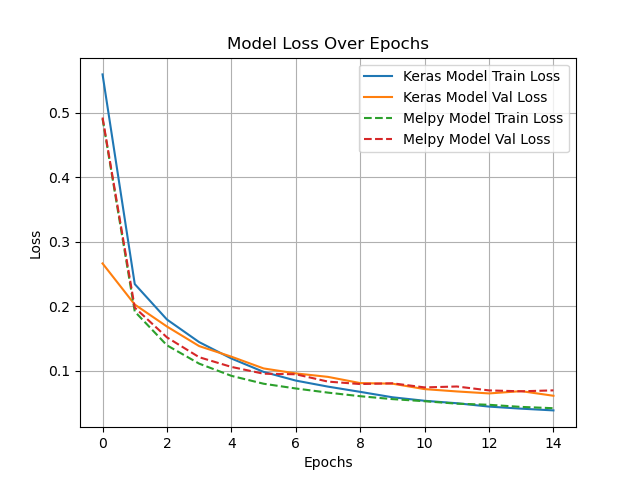
\includegraphics[width=\columnwidth]{images/mnist_loss_comparison.png}
\captionof{figure}{Comparaison du coût entre Melpy et Keras sur MNIST}
\hfill\break


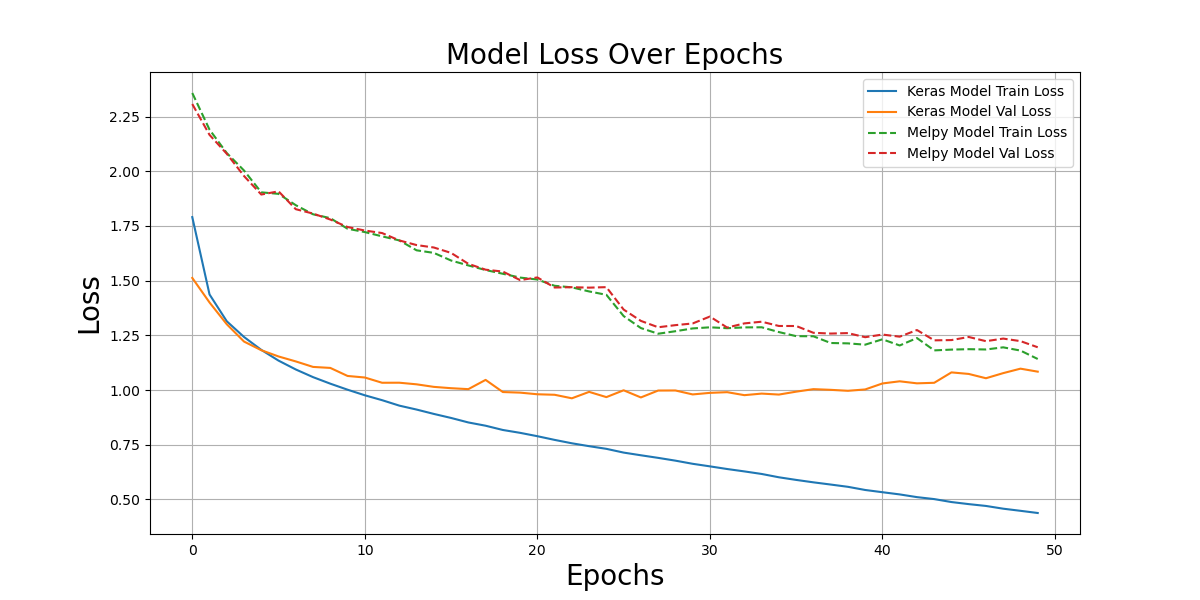
\includegraphics[width=\columnwidth]{images/cifar10_loss_comparison.png}
\captionof{figure}{Comparaison du coût entre Melpy et Keras sur CIFAR-10}
\hfill\break

Comme le montrent les Figures 16 et 17, les coûts sont meilleurs sur Keras que sur Melpy. Cela peut s’expliquer par une légère différence 
dans le calcul du gradient au niveau des couches de convolution. En effet, lors de tests comparant les résultats des opérations 
mathématiques implémentées dans Melpy avec celles de TensorFlow, la bibliothèque sur laquelle Keras s’appuie pour ses calculs, 
une différence moyenne allant de 0,4 à 0,6 a été observée entre les gradients de chaque valeur d’entrée. Cette différence est 
significative en raison du nombre élevé de valeurs impliquées. Par exemple, si l’on somme les erreurs du gradient d’une taille (1, 3, 32, 32), 
la somme des erreurs peut atteindre jusqu’à 1800, contre des valeurs proches de 0 pour les autres opérations sur lesquelles les tests ont été effectués. 
Toutefois, bien que cette différence mérite une étude plus approfondie, elle n’empêche pas un apprentissage tout aussi efficace. \\

On peut également relevé le temps d'execution qu'il a fallu à Keras sur les mêmes configurations que Melpy : \\

\scalebox{0.95}{
\begin{tabular}{l|c c|}
    \cline{2-3}
                                     & Melpy                  & Keras                                \\
    \hline
    \multicolumn{1}{|l|}{MNIST}      & 28min 22sec            & 01min 15sec                    \\
    \multicolumn{1}{|l|}{CIFAR-10}   & 04h 54min 52sec        & 10min 43sec                    \\

    \hline
\end{tabular}}
\captionof{table}{Durées des entrainements éffectués sur CIFAR-10 et MNIST} \\

La différence importante dans les temps d’exécution (voir Table 4) s’explique par les optimisations intégrées à Keras. 
La bibliothèque compile les modèles en code machine via TensorFlow, ce qui accélère l’exécution 
des opérations. De plus, Keras exploite efficacement le parallélisme sur les CPU, 
ce qui améliore de surcroit les performances des calculs.

En revanche, Melpy, dans son état actuel, n’intègre pas encore de telles optimisations. 
Ses opérations restent dépendantes de l’interprétation directe de Python, ce qui allonge 
les temps d’exécution. \\

\end{multicols}
{\color{gray}\hrule}
\begin{center}
\section{Conclusion}
\bigskip
\end{center}
{\color{gray}\hrule}
\vspace{0.5cm}

En conclusion, nous pouvons affirmer que ce projet a été un succès, ayant eu comme objectif d’implémenter 
la possibilité d’entraîner des CNNs avec Melpy. 

Nous avons observé une légère différence de performances 
entre notre implémentation et Keras, différence qui nécessitera une recherche plus approfondie pour être corrigée. 
Cependant, le principal axe d’amélioration réside dans l’optimisation des calculs. Cela pourrait être réalisé 
en intégrant d’autres bibliothèques telles que Numba, JAX ou Cython, permettant de compiler les modèles lors 
de l’entraînement et ainsi améliorer l’efficacité des calculs. \\
\bibliographystyle{plain}
\renewcommand\refname{Bibliographie}
\bibliography{references}

\end{document}